\begin{frame}{Categorical Data}
    In the previous section, we focused on numerical data. We now turn our attention to categorical data. 
    
    \vspace{24pt}This section includes more tools and language that we will use throughout the course. 
\end{frame}

\begin{frame}{Word Clouds}
    If we have text that we're interested in, we can turn words into categories. Here are the top seven words from the survey question about slaying a dragon:
    
    \begin{center}
        \begin{tabular}{l c}
		    Word    & Frequency \\ \hline
            sword   & 9 \\
            dragon  & 9 \\
            stab    & 6 \\
            kind    & 5 \\
            heart   & 4 \\
            fire    & 3 \\
            dont    & 3 
        \end{tabular}
    \end{center}
\end{frame}

\begin{frame}{Word Clouds}
    Here are a few things I did before finding the top words:
    \begin{itemize}
        \item Removed responses like "N/A" and "I don't know".
        \item Removed low-information words like "the" and "and".
        \item Removed punctuation.
        \item Converted all text to lowercase.
        \item Reduced words to their roots - "kindness" becomes "kind" - to group those words together.
    \end{itemize}
    
    \vspace{12pt}Now we're ready to create a word cloud out of the responses.
\end{frame}

\begin{frame}{Word Clouds}
    \begin{center}
        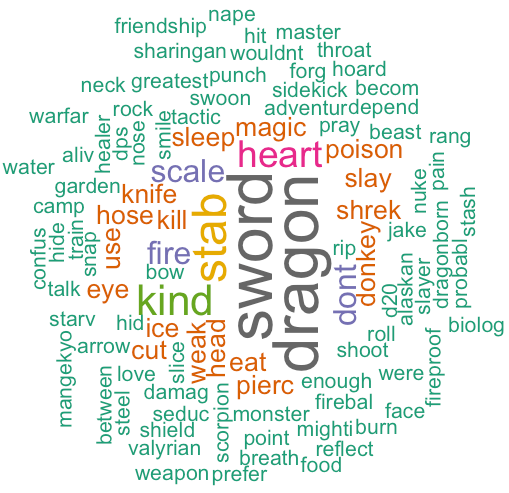
\includegraphics[scale=0.4]{images/dragonCloud.png}
    \end{center}
\end{frame}

\begin{frame}{Summary Tables}
    A basic \textbf{summary table} \textit{summarizes} a categorical variable by showing the frequency, or count, of each category.
    
    \begin{columns}[T] % align columns
        \begin{column}{.48\textwidth}
        %\color{red}\rule{\linewidth}{4pt}
        \begin{center}
        \begin{tabular}{l c}
		    \texttt{homeownership} & Count \\ \hline
		    Rent & 3858 \\ 
		    Mortgage & 4789 \\
		    Own & 1353 \\ \hline
		    Total & 10000 \\ \hline
        \end{tabular}
        \end{center}
        \end{column}%
        \hfill%
        \begin{column}{.48\textwidth}
        %\color{blue}\rule{\linewidth}{4pt}
        \begin{center}
        \begin{tabular}{l c}
		    \texttt{apptype} & Count \\ \hline
		    Individual & 8505 \\ 
		    Joint & 1495 \\ \hline
		    Total & 10000 \\ \hline
        \end{tabular}
        \end{center}
        \end{column}%
    \end{columns}
    \vspace{12pt}Note: \texttt{homeownership} refers to whether or not someone owns a home and \texttt{apptype} indicates whether a loan application was made individually or jointly.
\end{frame}

\begin{frame}{Bar Plots}
    A \textbf{bar plot} is a common way to visualize the information in a summary table. 
    \begin{center}
        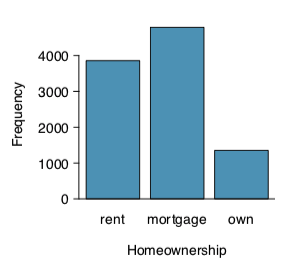
\includegraphics[scale=0.5]{images/barplot_freq.png}
    \end{center}
\end{frame}

\begin{frame}{Summary Tables: Proportions}
    We may occasionally prefer to see our data summarized by proportions (see the fractional breakdown of our data).
    
    \begin{columns}[T] % align columns
        \begin{column}{.48\textwidth}
        %\color{red}\rule{\linewidth}{4pt}
        \begin{center}
        \begin{tabular}{l c}
		    \texttt{homeownership} & Proportion \\ \hline
		    Rent & 0.3858 \\ 
		    Mortgage & 0.4789 \\
		    Own & 0.1353 \\ \hline
		    Total & 1.0000 \\ \hline
        \end{tabular}
        \end{center}
        \end{column}%
        \hfill%
        \begin{column}{.48\textwidth}
        %\color{blue}\rule{\linewidth}{4pt}
        \begin{center}
        \begin{tabular}{l c}
		    \texttt{apptype} & Proportion \\ \hline
		    Individual & 0.8505 \\ 
		    Joint & 0.1495 \\ \hline
		    Total & 1.0000 \\ \hline
        \end{tabular}
        \end{center}
        \end{column}%
    \end{columns}
\end{frame}

\begin{frame}{Bar Plots}
    We can again use a bar plot to visualize this information.
    \begin{center}
        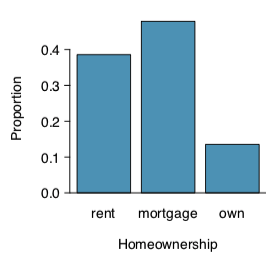
\includegraphics[scale=0.5]{images/barplot_prop.png}
    \end{center}
    This bar plot looks exactly the same as the one with frequencies! The only difference is in the numbers along the vertical axis.
\end{frame}

\begin{frame}{Pie Charts}
    Pie charts show the same information as bar charts, but are more difficult to discern details from. 
    \begin{center}
        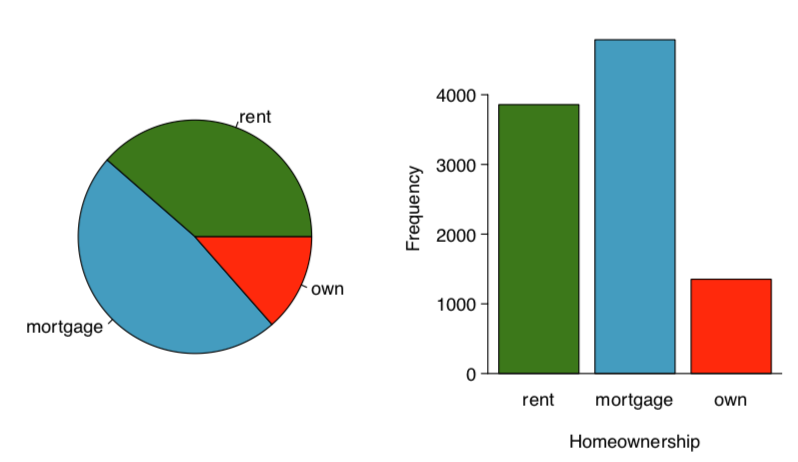
\includegraphics[scale=0.3]{images/piechart.png}
    \end{center}
    They are good for infographics but are not well-suited to technical writing.
\end{frame}

\begin{frame}{Contingency Tables}
    A \textbf{contingency table} is a table that summarizes two categorical variables. It looks something like this:
    \begin{center}
        \begin{tabular}{r l ccc r}
		& & \multicolumn{3}{c}{{\texttt{homeownership}}} & \\
        \cline{3-5}
		& & Rent & Mortgage & Own & Total  \\ 
        \cline{2-6}
        \multirow{2}{*}{{\texttt{apptype}}} 
        & Individual & 3496 & 3839 & 1170 & 8505 \\ 
  		& Joint & 362 & 950 & 183 & 1495 \\ 
        \cline{2-6}
  		& Total	& 3858 & 4789 & 1353 & 10000 \\
        \cline{2-6}
    \end{tabular}
    \end{center}
\end{frame}

\begin{frame}{Contingency Tables}
    \vspace{12pt}Contingency tables allow us to summarize two categorical variables together by breaking them down into subcategories. 
    \begin{center}
        \begin{tabular}{r l ccc r}
		& & \multicolumn{3}{c}{{\texttt{homeownership}}} & \\
        \cline{3-5}
		& & Rent & Mortgage & Own & Total  \\ 
        \cline{2-6}
        \multirow{2}{*}{{\texttt{apptype}}} 
        & Individual & 3496 & 3839 & 1170 & 8505 \\ 
  		& Joint & 362 & 950 & 183 & 1495 \\ 
        \cline{2-6}
  		& Total	& 3858 & 4789 & 1353 & 10000 \\
        \cline{2-6}
    \end{tabular}
    \end{center}
\end{frame}

\begin{frame}{Contingency Tables}
    Notice that the column of totals is the same as the summary table for \texttt{apptype} and the row of totals has the same information as the summary table for \texttt{homeownership}. 
    \begin{center}
        \begin{tabular}{r l ccc r}
		& & \multicolumn{3}{c}{{\texttt{homeownership}}} & \\
        \cline{3-5}
		& & Rent & Mortgage & Own & Total  \\ 
        \cline{2-6}
        \multirow{2}{*}{{\texttt{apptype}}} 
        & Individual & 3496 & 3839 & 1170 & 8505 \\ 
  		& Joint & 362 & 950 & 183 & 1495 \\ 
        \cline{2-6}
  		& Total	& 3858 & 4789 & 1353 & 10000 \\
        \cline{2-6}
    \end{tabular}
    \end{center}
\end{frame}

\begin{frame}{Row and Column Proportions}
    We may also want to examine the fractional breakdown of our contingency table data.
    \begin{itemize}
        \item \textbf{The row proportions are the row counts divided by the row total}.
        \item The column proportions are the column counts divided by the column total.
        \item The overall proportions are the counts divided by the total number of observations. 
    \end{itemize}
\end{frame}

\begin{frame}{Contingency Tables for Row Proportions}
    We can now convert our previous contingency table into a contingency table \textit{for the row proportions}:
    \begin{center}
        \begin{tabular}{r l ccc r}
		& & \multicolumn{3}{c}{{\texttt{homeownership}}} & \\
        \cline{3-5}
		& & Rent & Mortgage & Own & Total  \\ 
        \cline{2-6}
        \multirow{2}{*}{{\texttt{apptype}}} 
        & Individual & 0.411 & 0.451 & 0.138 & 1.000 \\ 
  		& Joint & 0.242 & 0.635 & 0.122 & 1.000 \\ 
        \cline{2-6}
  		& Total	& 0.386 & 0.479 & 0.135 & 1.000 \\
        \cline{2-6}
    \end{tabular}
    \end{center}
    
    \vspace{12pt}This breaks down each application type into home ownership status. We would say that, \textit{among individual applications}, 41.1\% are renters. 
\end{frame}

\begin{frame}{Contingency Tables for Row Proportions}
    \begin{center}
        \begin{tabular}{r l ccc r}
		& & \multicolumn{3}{c}{{\texttt{homeownership}}} & \\
        \cline{3-5}
		& & Rent & Mortgage & Own & Total  \\ 
        \cline{2-6}
        \multirow{2}{*}{{\texttt{apptype}}} 
        & Individual & 0.411 & 0.451 & 0.138 & 1.000 \\ 
  		& Joint & 0.242 & 0.635 & 0.122 & 1.000 \\ 
        \cline{2-6}
  		& Total	& 0.386 & 0.479 & 0.135 & 1.000 \\
        \cline{2-6}
    \end{tabular}
    \end{center}
    We can tell at a glance that this is for the \textit{row proportions} because all of the \textit{row totals} are 1. 
    
    \vspace{12pt}The rows are total breakdown of \texttt{homeownership}, so the bottom row of totals is the same as the home ownership summary table with proportions (see slide 15). They are \textit{not} the additive total for the row of proportions.
\end{frame}

\begin{frame}{Row and Column Proportions}
    \begin{itemize}
        \item The row proportions are the row counts divided by the row total.
        \item \textbf{The column proportions are the column counts divided by the column total}.
        \item The overall proportions are the counts divided by the total number of observations. 
    \end{itemize}
\end{frame}

\begin{frame}{Contingency Tables for Column Proportions}
    We can also convert our contingency table into a contingency table \textit{for the column proportions}:
    \begin{center}
        \begin{tabular}{r l ccc r}
		& & \multicolumn{3}{c}{{\texttt{homeownership}}} & \\
        \cline{3-5}
		& & Rent & Mortgage & Own & Total  \\ 
        \cline{2-6}
        \multirow{2}{*}{{\texttt{apptype}}} 
        & Individual & 0.906 & 0.802 & 0.865 & 0.851 \\ 
  		& Joint & 0.094 & 0.198 & 0.135 & 0.150 \\ 
        \cline{2-6}
  		& Total	& 1.000 & 1.000 & 1.000 & 1.000 \\
        \cline{2-6}
    \end{tabular}
    \end{center}
    
    \vspace{12pt}This breaks down each home ownership status into application types. We would say that, \textit{among renters}, 90.6\% filled out an individual loan application. 
\end{frame}

\begin{frame}{Contingency Tables for Row Proportions}
    \begin{center}
        \begin{tabular}{r l ccc r}
		& & \multicolumn{3}{c}{{\texttt{homeownership}}} & \\
        \cline{3-5}
		& & Rent & Mortgage & Own & Total  \\ 
        \cline{2-6}
        \multirow{2}{*}{{\texttt{apptype}}} 
        & Individual & 0.906 & 0.802 & 0.865 & 0.851 \\ 
  		& Joint & 0.094 & 0.198 & 0.135 & 0.150 \\ 
        \cline{2-6}
  		& Total	& 1.000 & 1.000 & 1.000 & 1.000 \\
        \cline{2-6}
    \end{tabular}
    \end{center}
    We can tell at a glance that this is for the \textit{column proportions} because all of the \textit{column totals} are 1. 
    
    \vspace{12pt}The rows are the total breakdown of \texttt{apptype}, so the bottom row of totals is the same as the application type ownership summary table with proportions (see slide 15). They are \textit{not} the additive total for the column of proportions. 
\end{frame}

\begin{frame}{Contingency Tables for Row Proportions}
    \begin{center}
        \begin{tabular}{l ccc r}
		& Rent & Mortgage & Own & Total  \\ 
        \cline{2-5}
        Individual & 0.906 & 0.802 & 0.865 & 0.851 \\ 
  		Joint & 0.094 & 0.198 & 0.135 & 0.150 \\ 
        \cline{2-5}
  		Total	& 1.000 & 1.000 & 1.000 & 1.000 \\
        \cline{2-5}
    \end{tabular}
    \end{center}
    \begin{itemize}
        \item We can use these contingency tables to check for an association between home ownership and loan type.
        \item Notice that, among individual applicants, 90.5\% rent, but only 80.2\% have a mortgage.
    \end{itemize}
\end{frame}

\begin{frame}{Contingency Tables for Row Proportions}
    \begin{center}
        \begin{tabular}{l ccc r}
		& Rent & Mortgage & Own & Total  \\ 
        \cline{2-5}
        Individual & 0.906 & 0.802 & 0.865 & 0.851 \\ 
  		Joint & 0.094 & 0.198 & 0.135 & 0.150 \\ 
        \cline{2-5}
  		Total	& 1.000 & 1.000 & 1.000 & 1.000 \\
        \cline{2-5}
    \end{tabular}
    \end{center}
    \begin{itemize}
        \item If there is no association, the proportions will be (approximately) the same across the row.
        \item We say that loan types \textit{vary between} different \textbf{levels} of home ownership. 
        \item (Using the column proportions, we can also say that home ownership status varies between levels of loan type.)
    \end{itemize}
\end{frame}

\begin{frame}{Example: Student Survey}
    Let's look at a contingency table for some of our survey data.
    
    \begin{center}
        \begin{tabular}{r l cccc r}
		& & \multicolumn{4}{c}{{\texttt{Year}}} & \\
        \cline{3-6}
		& & Sophomore & Junior & Senior & Other & Total  \\ 
        \cline{2-7}
        \multirow{2}{*}{{\texttt{Want}}} 
        & 1 & 1 & 0 & 2 & 1 & 4 \\ 
  		& 2 & 0 & 4 & 3 & 1 & 8 \\ 
  		& 3 & 1 & 11 & 1 & 0 & 23 \\ 
  		& 4 & 7 & 10 & 8 & 1 & 26 \\ 
  		& 5 & 0 & 3 & 1 & 0 & 4 \\ 
        \cline{2-7}
  		& Total	& 9 & 28 & 25 & 3 & 65 \\
        \cline{2-7}
    \end{tabular}
    \end{center}
    
    Is there a relationship between year and desire to take this course?
\end{frame}

\begin{frame}{Example: Student Survey}
    It's hard to tell! Let's look at whether there is a change in \texttt{want} by \texttt{year} (does want vary between levels of year).
    
    \begin{center}
        \begin{tabular}{r l cccc r}
		& & \multicolumn{4}{c}{{\texttt{Year}}} & \\
        \cline{3-6}
		& & Sophomore & Junior & Senior & Other & Total  \\ 
        \cline{2-7}
        \multirow{2}{*}{{\texttt{Want}}} 
        & 1 & 0.11 & 0.00 & 0.08 & 0.33 & 0.06 \\ 
  		& 2 & 0.00 & 0.14 & 0.12 & 0.33 & 0.12 \\ 
  		& 3 & 0.11 & 0.39 & 0.44 & 0.00 & 0.35 \\ 
  		& 4 & 0.78 & 0.36 & 0.32 & 0.33 & 0.40 \\ 
  		& 5 & 0.00 & 0.11 & 0.04 & 0.00 & 0.06 \\ 
        \cline{2-7}
  		& Total	& 1.00 & 1.00 & 1.00 & 1.00 & 1.00 \\
        \cline{2-7}
    \end{tabular}
    \end{center}
    
    Is there a relationship between year and desire to take this course?
\end{frame}

\begin{frame}{Example: Student Survey}
    What if we looked at whether there is a change in \texttt{year} by \texttt{want} (does year vary between levels of want)?
    \begin{itemize}
        \item We should still see a relationship.
        \item It makes sense to think about whether year affects your desire to take this course.
        \item However, it probably doesn't make sense to think about whether desire to take this course affects your year in school.
        \begin{itemize}
            \item In this scenario, you'd have to have done something extreme like taken a year off and fallen behind just because you really didn't want to take this course. Hopefully that's not the case!
        \end{itemize}
    \end{itemize}
\end{frame}

\begin{frame}{Two-Variable Bar Plots}
    \begin{itemize}
        \item We can extend our bar plots to help visualize the information in a contingency table by creating
        \begin{itemize}
            \item \textbf{Stacked bar plots}.
            \item \textbf{Side-by-side bar plots}.
        \end{itemize} 
        \item A stacked bar plot takes our one-variable bar plot and breaks up the bars to show a second variable.
        \item A side-by-side bar plot takes our one-variable var plot and splits each bar into two side-by-side bars.
    \end{itemize}
\end{frame}

\begin{frame}{Side-By-Side Bar Plots}
    \begin{center}
        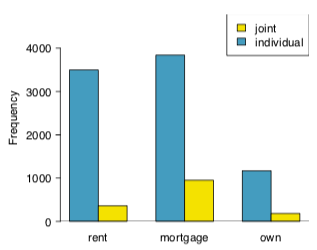
\includegraphics[scale=0.45]{images/sidebar.png}
    \end{center}
    This side-by-side bar plot shows home ownership with loan application type. Here, we're breaking the data into six categories and giving each one a bar.
\end{frame}

\begin{frame}{Stacked Bar Plots}
    \begin{center}
        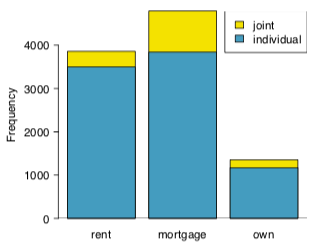
\includegraphics[scale=0.45]{images/stackedbar.png}
    \end{center}
    This stacked bar plot shows home ownership broken down by loan application type. 
    
    \vspace{12pt}In both plots, it is easy to see that there are fewer people who own their homes and fewer people applying for joint loans. 
\end{frame}

\begin{frame}{Stacked Bar Plots: Frequencies}
    \begin{center}
        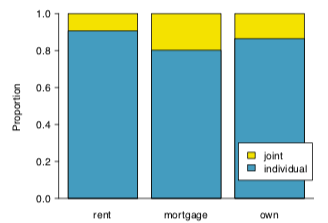
\includegraphics[scale=0.45]{images/stackedbarstd.png}
    \end{center}
    \begin{itemize}
        \item Same information, but standardized based on home ownership.
        \item This is a visualization of the frequency-based contingency table for loan types varying between levels of home ownership (slide 30). 
        \item Now we can see that the two variables are associated.
    \end{itemize}
\end{frame}

\begin{frame}{Example: Student Survey Data}
    Let's turn our contingency table into a stacked bar plot:
    \begin{center}
        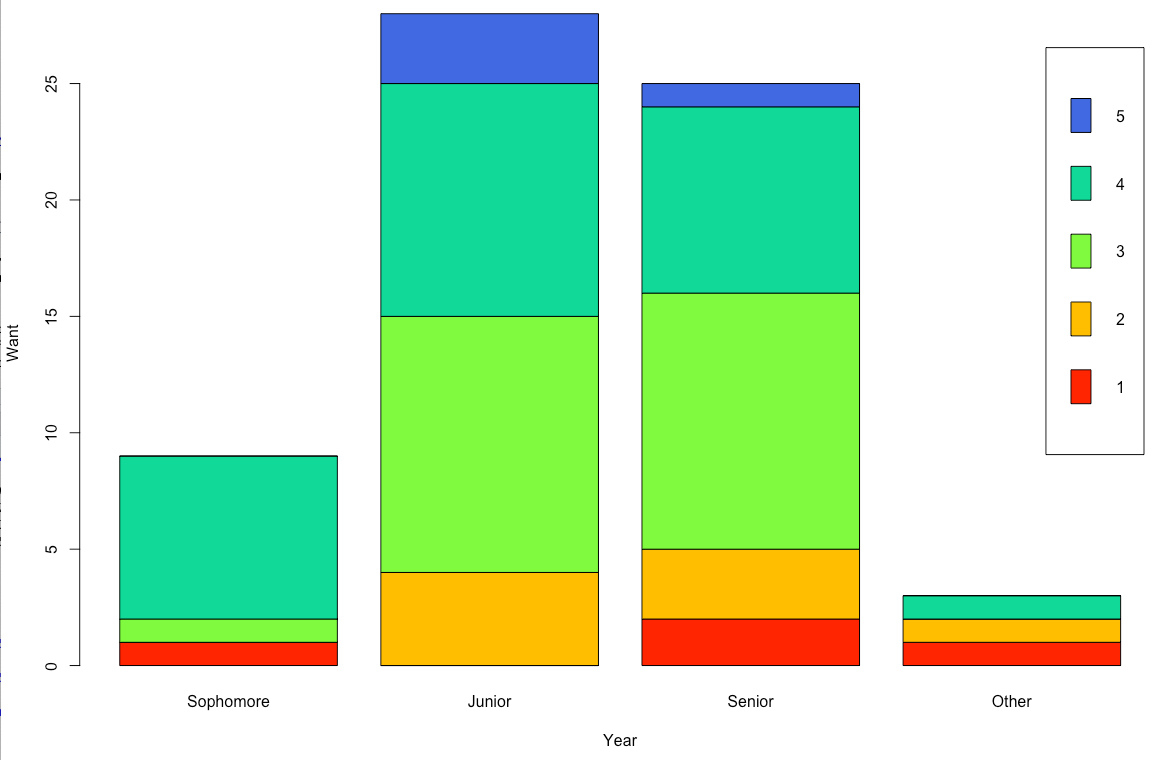
\includegraphics[scale=0.18]{images/exbarplot.png}
    \end{center}
    Here, we can see that most of you are juniors and seniors (and that there's a decent spread of how much you want to be here).
\end{frame}

\begin{frame}{Example: Student Survey Data}
    Let's do the same with the proportion-based table:
    \begin{center}
        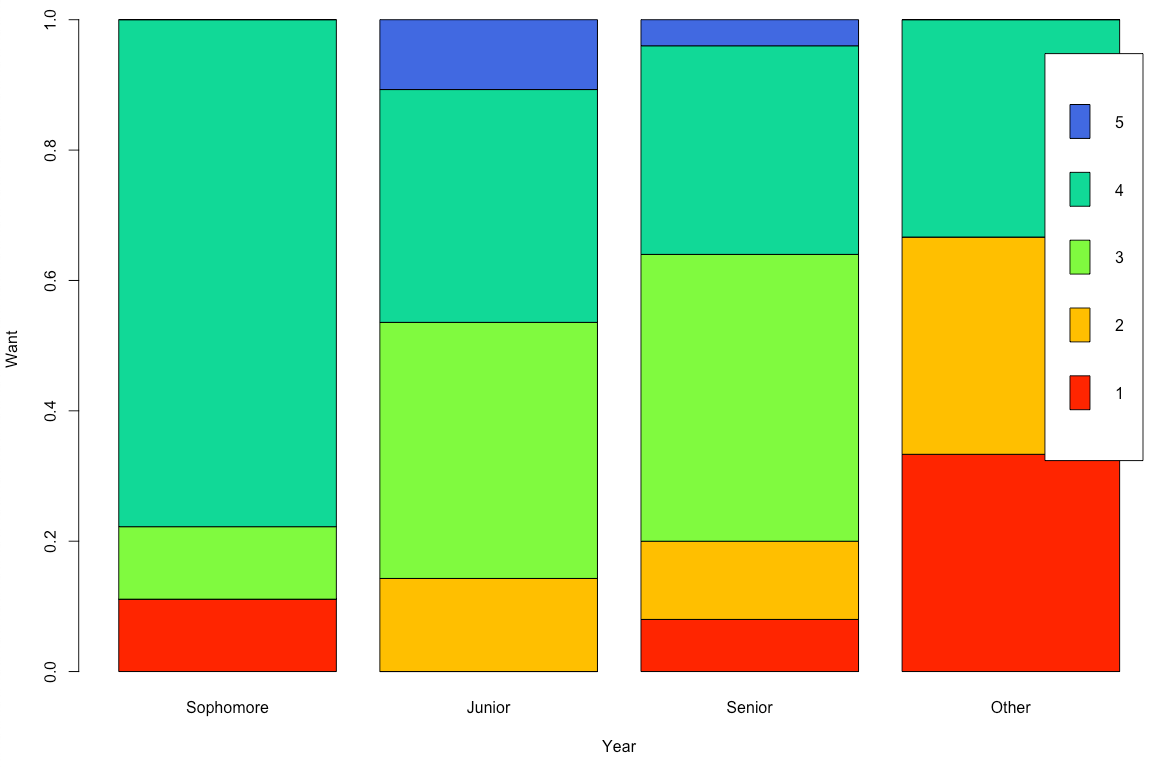
\includegraphics[scale=0.2]{images/exbarplot2.png}
    \end{center}
    Now we can quickly visualize the differences between the years.
\end{frame}

\begin{frame}{Mosaic Plots}
    \begin{center}
        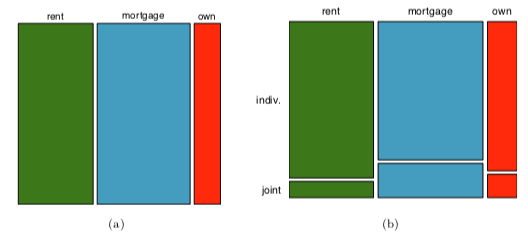
\includegraphics[scale=0.5]{images/mosaic.png}
    \end{center}
    \noindent(a) is a one-variable mosaic plot for \texttt{homeownership}.\\
    \noindent(b) is a two-variable mosaic plot for \texttt{homeownership} and \texttt{app\_type}.
\end{frame}

\begin{frame}{Mosaic Plots}
    \begin{itemize}
        \item Mosaic plots look a lot like bar plots, but now the \textit{widths} of the bars depend on the group sizes.
        \item For two-variable mosaic plots, the boxes from the one-variable mosaic plot are divided up using the second variable.
        \item Now, the \textit{heights} of the boxes also depend on group sizes.
        \item Thus, mosaic plots use \textit{area} to represent the number of cases in each category.
    \end{itemize}
\end{frame}

\begin{frame}{Example: Student Survey Data}
    \begin{center}
        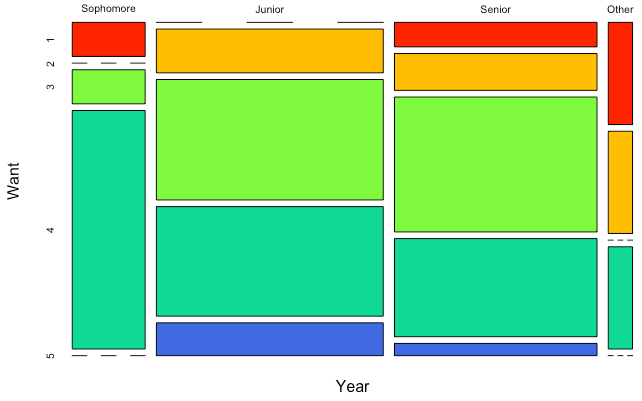
\includegraphics[scale=0.35]{images/mosaicex.png}
    \end{center}
    We can again see that there are more juniors \& seniors in the class and that sophomores are more likely to want to take this course beyond its being a requirement. 
\end{frame}

\begin{frame}{Comparing Numerical Data Across Groups}
    \begin{itemize}
        \item Our question of interest often involves comparing numerical data across categories.
        \item Whenever we are interested in comparing some numeric outcome across treatment groups, this is our goal!
        \item In general, these comparisons require that we make side-by-side or stacked versions of our data visualization techniques for numerical data.
    \end{itemize}
\end{frame}

\begin{frame}{Side-By-Side Box Plots}
    \textbf{Side-by-side box plots} are standard tools for visualizing numerical data broken down into categories.
    
    \begin{center}
        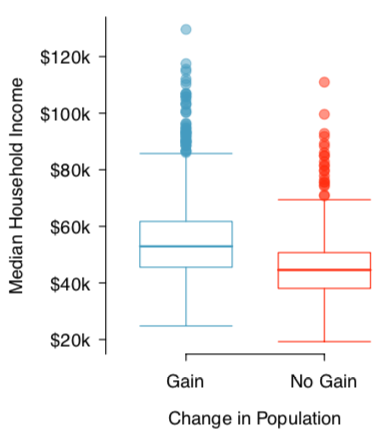
\includegraphics[scale=0.35]{images/sidesidebox.png}
    \end{center}
\end{frame}

\begin{frame}{Example: Student Survey Data}
    Let's look at how number of pets differs between year: 
    \begin{center}
        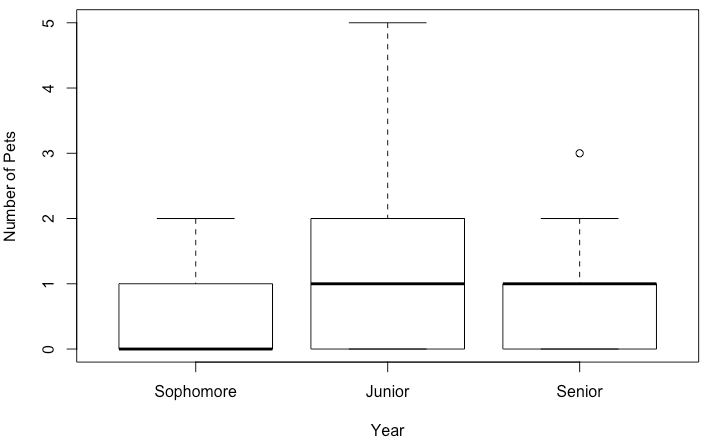
\includegraphics[scale=0.3]{images/petsyearbox.png}
    \end{center}
    Juniors have a larger IQR and longer whiskers, suggesting that they have a larger spread in number of pets.
\end{frame}

\begin{frame}{Hollow (or Stacked) Histograms}
    \begin{center}
        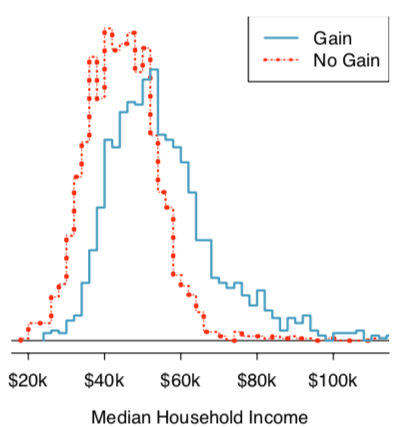
\includegraphics[scale=0.33]{images/hollowhists.png}
    \end{center}
    Hollow histograms are a little bit harder to read, but they allow us to visualize what two distributions look like when layered on top of each other.
\end{frame}
